\chapter{Historical Development}\label{c:History}
\section{Introduction}
\subsection{Overview of chapter}
There is a clear and well-documented trend for languages spoken in the Himalayan region to grammatically mark epistemic meaning in a variety of ways, as has been discussed in Chapter \ref{c:Description}. While it is generally understood that epistemic marking spreads areally and tends to occur in geographic hotspots rather than along genealogical lines \cites[288]{Aikhenvald2004}{SanRoque2012}{Verhees2018}, there remains a question, at least in the Himalayas, as to the point of origin of the epistemic-marking sprachbund. That is, if epistemic marking has spread areally, where did it originate and how did it spread? Alternatively, is the widespread nature of the epistemic marking---which, while generally occuring within the \lfam\ family---crosses subfamily boundaries, in fact due to areal diffusion, or is it better attributed to inheritance and convergent evolution of languages as a result of some other, extralinguistic factors?

This chapter investigates these questions using the typological observations presented in \cref{c:Description}. It compares the contemporary geographic distribution of types of epistemic marking with historical extralinguistic factors that would have affected language contact and areal influence such as religious, economic, and political relationships. In doing so, it finds a correlation between the presence of complex epistemic systems and contact with Tibetic languages, suggesting two possibilities. Firstly, epistemic marking may be a relatively more recent innovation in the \lfam\ family, having spread throughout the region using the spread and subsequent economic, political, and religious influence of the Tibetan Empire as a conduit. Alternatively, epistemic marking may predate the Tibetan Empire, potentially having been inherited from a proto-language, but lost in areas in contact with non-\lfam\ languages. However, that with the data currently available, and more importantly with the lack of ability to reconstruct forms and assess historical social situations in great detail, it is not possible to take a clear stance on either of the presented hypotheses.

Section \ref{ss:History:Schema} will present the schema used to categorise the languages into discrete groups for the purpose of mapping trends based on typologies discussed in Section \ref{sss:Description:GroupSize}, while Section \ref{s:History:Map} presents this map, along with some initial observations. Section \ref{s:History:Contact} will detail the possible extra-linguistic historical factors that may have influenced the development of epistemic marking across the \lfam\ languages, dividing the \lfam-speaking area into eight regions and investigating them individually. It finds generally widespread contact with Tibetic speakers across combinations of economonic, political, or religious domains, excepting areas further afield or blocked by mountains such as the Myanmar area. Section \ref{s:History:Correlations} will take factors presented in Section \ref{s:History:Contact} and propose two possible explanations given above for the development of epistemic marking in the family in detail. The key pieces of knowledge we lack---namely information on the time depth of the development of evidential forms in various languages, the historical prevalence of multilingualism in Tibetic-adjacent communities, historical community sizes, and evidence of clearly cognate forms---are discussed in Section \ref{s:History:FurtherFactors}. Section \ref{s:History:CaseStudies} presents a number of specific case studies that provide more specific insights into the historical possibilities for the development of these systems. While it is possible to claim that either one of the presented hypotheses is the ``correct'' one, as is so often the case with language, it seems likely given the evidence that will be discussed that the reality is a more complex mix of the two, with different types of language contact occurring over different time periods.

\subsection{Schematising epistemics}\label{ss:History:Schema}
In order to assess large-scale patterns or trends across the languages surveyed, the data must be grouped into categories according to their epistemic systems. Of course, there is no way to do this without losing substantial amounts of nuance and detail from the data. For this purpose, this section will assess the data using a typological schema developed from the observations presented in Section \ref{sss:Description:GroupSize}, grouping epistemic systems in terms of their size. A two-tier distinction was presented in Section \ref{sss:Description:GroupSize}, dividing systems into Complex and Single Term systems, which were in turn divided into Scattered and Paradigmatic, and A3 (Reportative) systems and others, respectively.

For the most part, the schema used here has sufficient dividing the systems into cohesive groups in order to draw reasonable conclusions. There are, of course, some cases where the detail lost in this schema does provide deeper insights into possible historical development routes, and as such specific data in select examples will be presented in Section \ref{s:History:CaseStudies}. Similarly, the division between paradigmatic and scattered systems can be blurry. In schematising the data for this representation, judgements had to be made as to how to categorise the data that are not necessarily completely clear-cut or doubtless. That is, while the typology of systems appearing either paradigmatic or scattered is not untrue, in practice the scale has a more extensive gradient than expected. For example, even a language treated as an archetypal example of a paradigmatic system such as Kurtöp (\cite[East Bodish: Bhutan, ][]{Hyslop2020Kurtop}) has multiple paradigms marking epistemic meaning across various parts of the grammar, namely verbal morphology and copulas. A number of languages also have systems of either clause or sentence final particles (e.g., Dhimal \cite{King2009}, Kadu \cite{Sangdong2012}, Namuzi \cite{Pavlik2017}, Munya \cite{Bai2019}, Poumai Naga \cite{Veikho2021}). The prevalence of these particles across the family has been noted prior \cite{DeLancey2011}, and often mark functions beyond epistemics. Whether or not these sets of particles can be considered a single paradigm is requires a depth of consideration that cannot not be answered here due to space limitations, though is discussed in Section \ref{sss:Discussion:Paradigmatic}. Considering that they fill the same grammatical slot, however, they have been classified here as paradigmatic provided that they have multiple epistemic forms within the set of final particles.

The schema organises languages into five categories:
\begin{itemize}
    \item Complex Epistemic Systems
    \begin{itemize}
        \item Paradigmatic
        \item Scattered
    \end{itemize}
    \item Single Term Systems
    \begin{itemize}
        \item A3 Systems
        \item Other Systems
    \end{itemize}
    \item No Epistemic Marking
\end{itemize}
\subsubsection{Complex Epistemic Systems}
The first category contains epistemic systems with multiple possible epistemic bases encoded throughout the grammar. That is, there is a distinction between multiple epistemic bases, either in a single paradigm, or dispersed across various grammatical domains (paradigmatic or scattered). To some extent, this category is defined against the next (Single Term Systems, divided into A3 systems and others) by exclusion, and is clear opposition to the last (No Epistemic Marking). Systems that fall into this category include the well-described system in Lhasa Tibetan \cite{DeLancey2017Tibetan}, and Akha \cite{Thurgood1986}.
\subsubsection{Single Term Systems}
Single Term Systems, as established in Section \ref{sss:Description:GroupSize}, refer to systems which mark either a single epistemic base, or a single epistemic contrast depending on the analysis. The category is further divided into two, A3 systems and others.

``A3'' systems as described in \citeA{Aikhenvald2004} mark only reported evidence. These systems are separate as they represent a sizeable subset of the languages surveyed. Their prevalence in \lfam\ languages is by no means a fact that has gone unnoticed in the literature, \citeA{Gawne2021} provides an in-depth analysis of reported evidence across the family (with a far more detailed survey than managed in this thesis), and finds it to be prevalent across the family, as part of a larger paradigm or by itself.

Finally, other single term systems, as with A3 systems, mark only one epistemic base. They are separated from A3 systems as no single other distinction is prevalent enough to warrant being grouped separately. That is, while these are formally similar to A3 systems, the widespread nature of sole marking of reportative evidence means that they are worth assessing separately. 
\subsubsection{No Epistemic Marking}
Finally, a number of languages surveyed showed no evidence of epistemic marking at all, and are grouped as such. The largest group of these languages is the Sinitic branch, the majority of which do not appear to exhibit any morphologically marked epistemic meaning (aside maybe from epistemic modality). Because epistemic marking is so notably absent from the subfamily (with the notable exception of Wutun, to be discussed in full in Section \ref{s:History:Correlations}), these languages have largely been excluded from this section of the survey, and from the maps presented in this chapter.

\section{Mapping the data}\label{s:History:Map}
In order to efficiently visualise the distribution of epistemic marking in the \lfam\ family, and subsequently establish any geographic patterns and assess their potential origins, the data has been overlaid on a map of the Himalayas and surrounds. The specifics of the creation of the map are discussed in Section \ref{ss:History:Map}, while some initial observations will be made in Section \ref{ss:History:MapPatterns}.

\subsection{Map}\label{ss:History:Map}
\begin{figure}
    \caption{A survey of Trans-Himalayan languages by type of Evidential System}
    \centering
    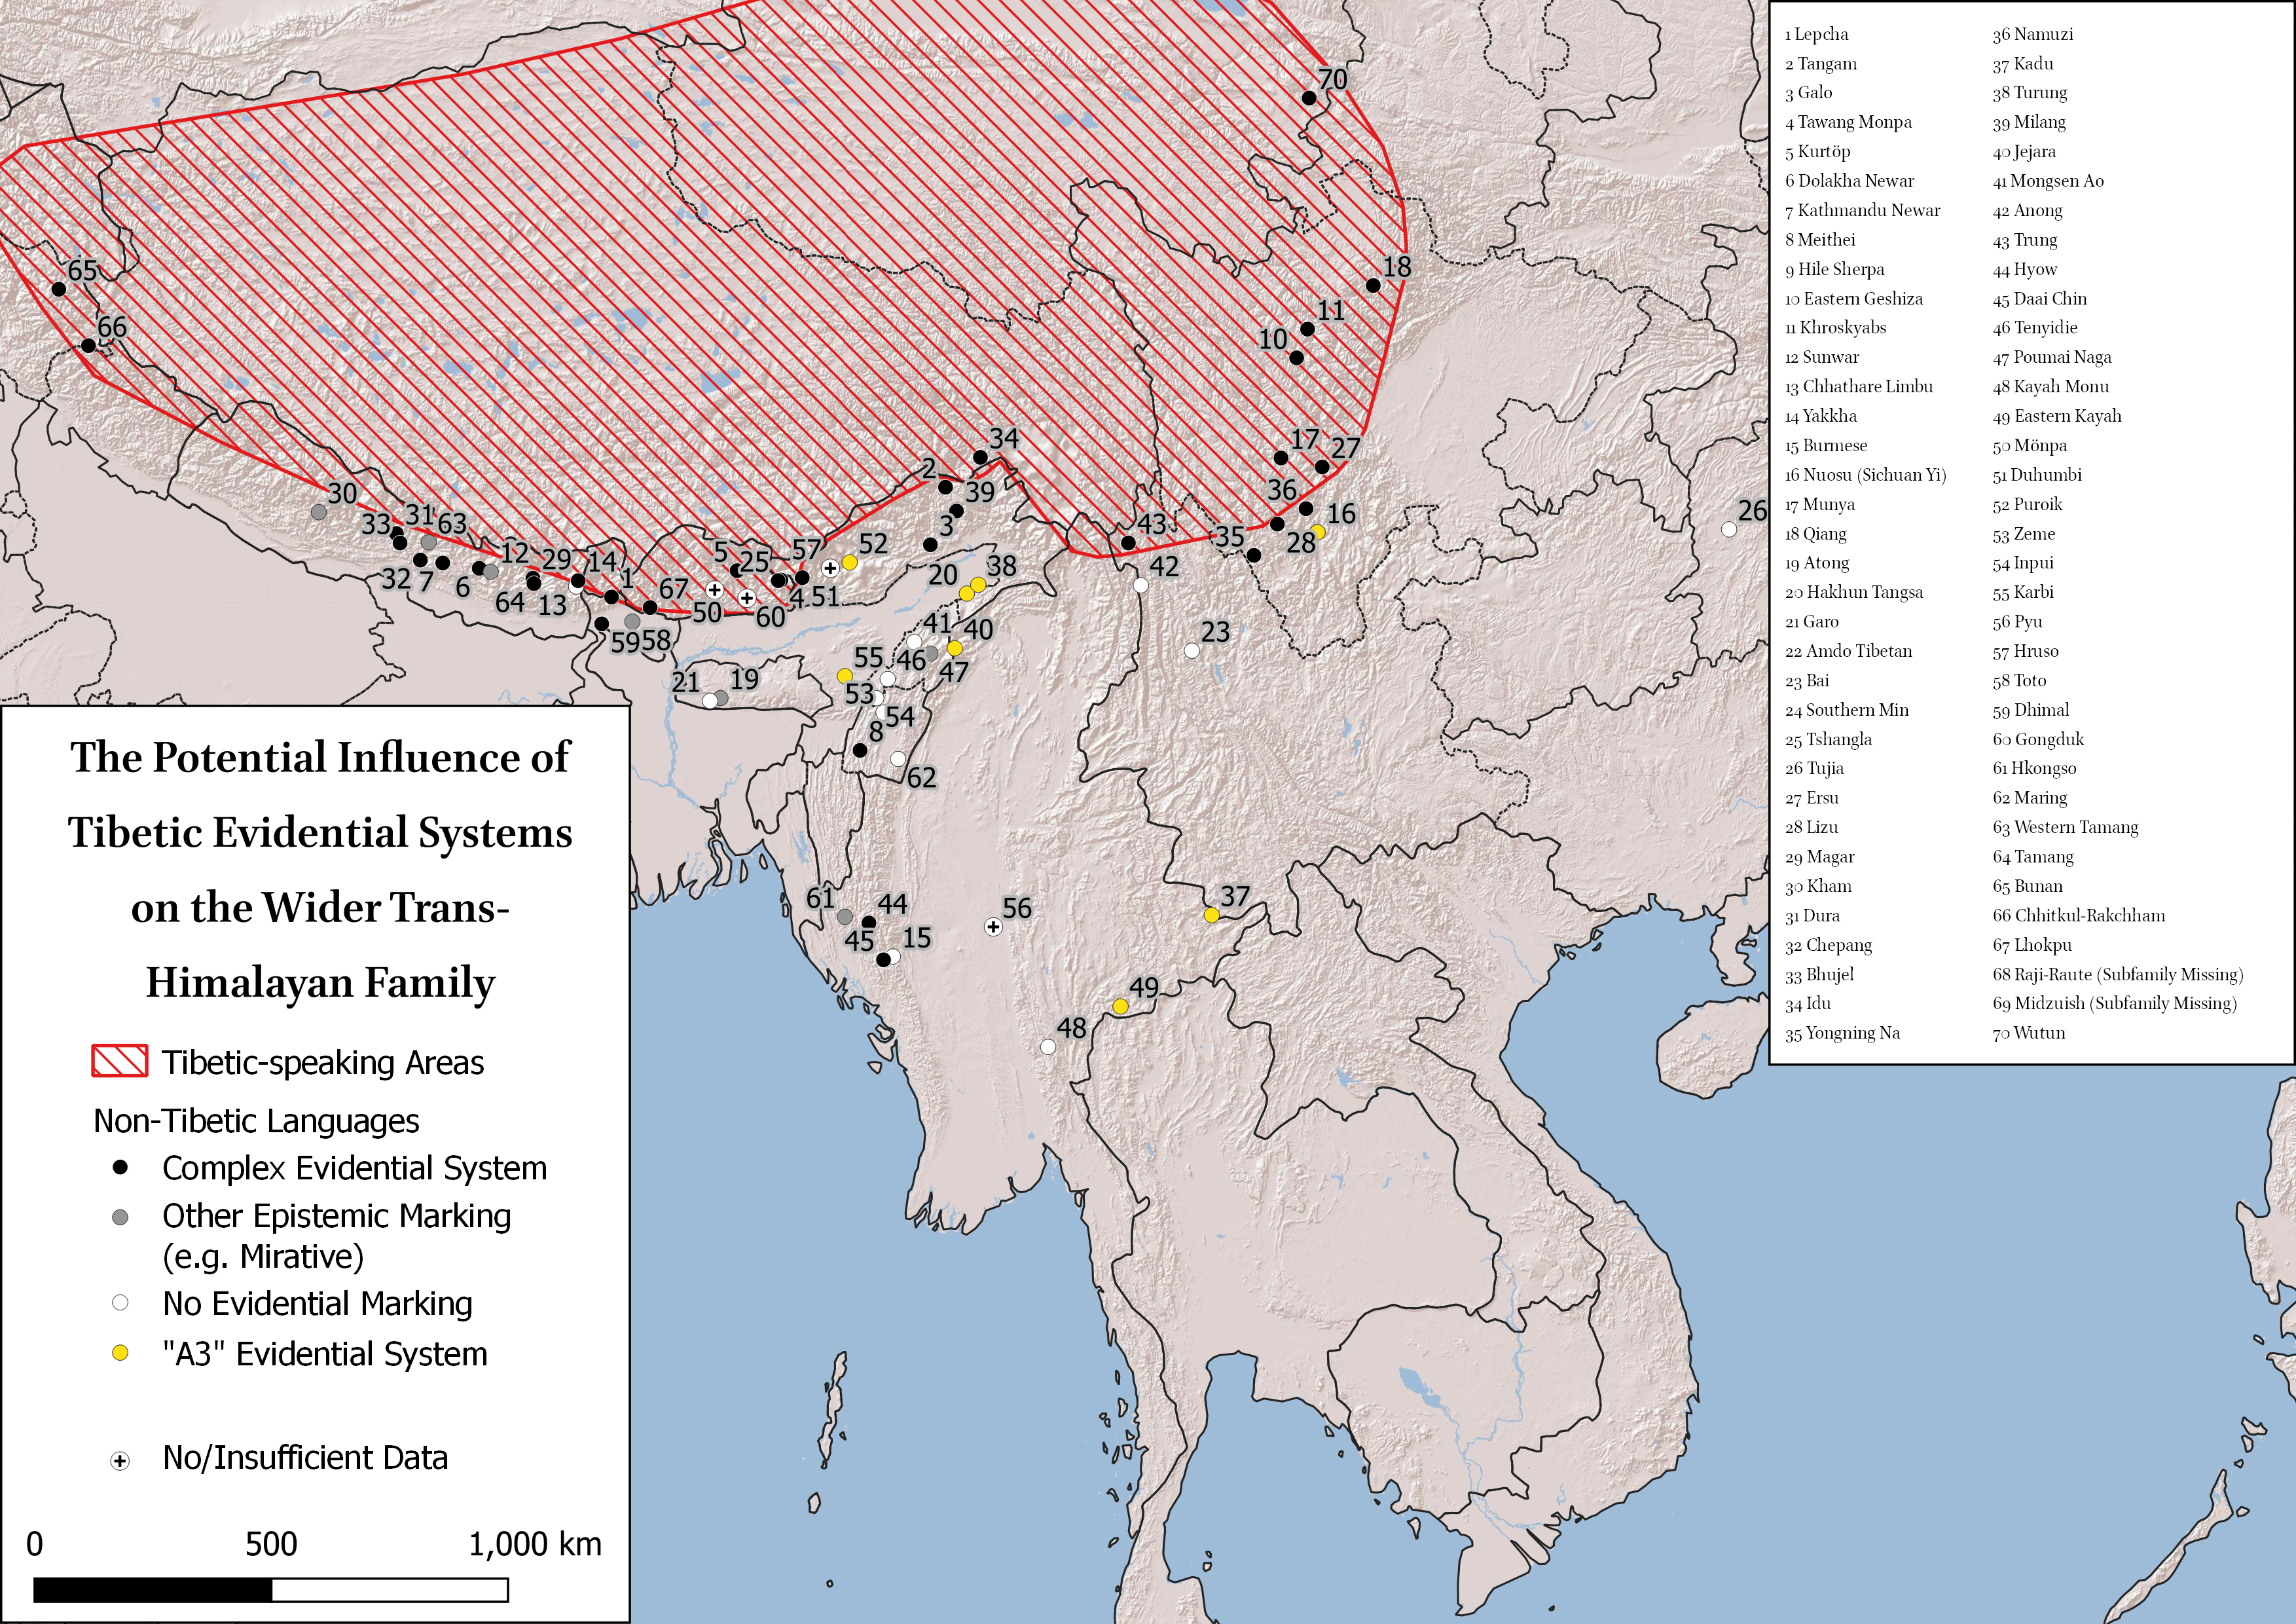
\includegraphics[width=\textwidth]{Tibetic Source Single Page Small.png}
    \label{map:EvidentialityMap}
\end{figure}
\figref{map:EvidentialityMap} shows the geographic distribution of a survey of languages, colour-coded according to their use of evidentiality. The map shows an approximation of the overall area in which Tibetic languages are spoken. Languages, of course, are not spoken in a single point, but are spread across variously sized areas. In some cases, at the scale of the map, a single point is sufficient to represent the total area in which a given language is spoken, though in many other cases, the points simply represent a centre point of the language's distribution. The coordinates of all points were taken from Glottolog \cite{glottolog}. These point data stem from a wide variety of different sources, including other databases such as Ethnologue and WALS, published data, and personal communication. For these reasons, they are used here as an approximation that is suitable for the very general assessment of typological distribution, but would perhaps not be rigorous enough for close geographical work on a single language or subfamily. 

Initial data for the Tibetic-speak area was similarly taken from Glottolog, with the full set of point data for languages within the ``Early Old Tibetan'' subgroup converted to a polygon (excluding the point representing Gyalsumdo, which at the time of analysis was seemingly erroneously located in central India rather than Nepal). This was then manually edited to more accurately represent the boundary regions as per the highly detailed survey in \citeA{Tournadre2023}, as well as some more specific sources such as \citeA{Post2017a}, which references some Tibetic speakers seemingly not noted in \citeA{Tournadre2023}.

\subsection{Discussion, initial patterns}\label{ss:History:MapPatterns}
It is clear at first glance in \figref{map:EvidentialityMap} that there are a significant number of black points (that is, complex evidential systems, either scattered or paradigmatic) near Tibetic-speaking areas, and fewer such points further away. This is, however, not a perfect correlation. A number of languages with complex evidential systems have been identified in the survey further afield. These languages, Meithei \cite{Chelliah1997}, Hyow \cite{Zakaria2018}, and Daai Chin \cite{SoHartmann2009}, will be discussed in Section \ref{ss:History:Outliers}. Similarly, there are some languages in proximity to Tibetic-speaking areas without complex evidential systems, such as Western Tamang \cite{Regmi2018} and Dhimali \cite{King2009}. In terms of the other categories, there is also a cluster of A3 reportative systems and languages entirely lacking epistemic marking in North-East India, specifically in and around the state of Nagaland. This cluster is in part attributable to the linguistic diversity in the region. Many of the so-called fallen leaf subfamilies \cite{VanDriem2014} are spoken in this area, often overlapping, and as a result there are many languages sampled. It is, however, of note how few of these contain of complex epistemic-marking systems. The possible reasons for this will be discussed at length below, namely in Section \ref{s:History:Correlations}, but it certainly appears that whatever areal or other process that has led to the widespread prevalence of complex epistemic-marking systems higher in the Himalayas and across the Tibetan Plateau has not occurred here, at least not to the same extent (given there are still languages with complex systems such those mentioned above).

\section{Historical Contact}\label{s:History:Contact}
\subsection{Introduction}
This section will investigate the historical contact across the Himalayas, in particular focussing on the contact between Tibetic-speaking groups and their neighbours. It will assess various groups' historical social, economic, and cultural connections to historical Tibet and non-\lfam-speaking groups, and use that to consider any possible sociolinguistic influence. In order to make this a more manageable undertaking, the map is divided into eight regions. These regions are intended to represent various cultural and linguistic macro-areas, though are not particularly academically informed. The regions are as follows:
\begin{enumerate}
    \item Bhutan, Sikkim
    \item Arunachal Pradesh 
    \item North-East India\footnote{I originally had thought to group Bhutan, Arunachal Pradesh, and the rest of North-East India together, however it became clear that the three regions have very different histories in terms of their trade and contact with other groups. These differences will be made clear in their respective sections.}
    \item Central Himalayas, Nepal
    \item Western Himalayas
    \item Yunnan, Sichuan
    \item Northern Flank of Tibet
    \item Myanmar
\end{enumerate}
\subsection{Bhutan, Sikkim}
The non-Tibetic languages of Bhutan and Sikkim have been in close contact with Tibetic languages for an extended time period. While it may initially seem clear that, in both having major Tibetic languages spoken in with social prestige throughout the regions,\footnote{Though Denjongke has declined in usage substantially} and in the dominance of Tibetan Buddhism in both areas, there has been a great amount of contact and influence from Dzongkha and Denjongke on non-Tibetic languages, it is worth investigating the time-depth of these languages, and the time-frame over which they spread and gained their modern-day influence. 

The Tibetic-speaking Bhutanese group, Ngalops, appear to have first arrived in Western Bhutan at some point prior to the ninth century \cite{VanDriem2001b}, and Tibetan Buddhism began to spread in the region it appears from the construction of the Kyichu and Jampa Lhakhangs in the seventh century \cite{Phuntsho2014}. The precise history of the Tibetic-speakers in Bhutan, however, remains more obscure. In Sikkim, the timing of the arrival of Tibetic-speakers is similarly unclear \cites{Spengen2010}{Yliniemi2021}, though in both cases it appears that the region was under the rule of the Tibetan Empire during the ninth century \cite{Schaik2013}. At the very least, it is sufficient to say that there has been a great deal of contact between Tibetic-speaking and non-Tibetic-speaking people throughout the last millennium.

\subsection{Arunachal Pradesh}\label{ss:History:Arunachal}
In contrast to Bhutan and Sikkim, where Tibetic languages and Tibetan Buddhism are widespread, there appears to have been relatively small amount influence or contact between the majority of the area that today constitutes Arunachal Pradesh\footnote{Tani-speaking areas as well as a number of smaller subfamilies including Hrushish, Midzuish, Digarish, and Kho-Bwa} and the neighbouring powers of Tibet and the Ahom Kingdom. 

\citeA{Nyori1993} notes a good trade relationship between some Tani groups and the Ahom Kingdom, particularly in the Kingdom's later years, as well as more substantial contact between the Ahoms and the Mising people, a Tani group who at some point migrated to the lowlands of the Brahmaputra. This contact, at least outside of the Mising people, does not appear to have had any major influence on these groups. Traditional religions have remained widespread and there is no clear linguistic influence from the Tai Ahom language (Mark Post p.c. 2022). Nyori also reports contact between the Tani people from Central Northern Arunachal Pradesh and Tibetic-speakers, both in the form of Tibetans and Khambas and Membas, two smaller Tibetic-speaking groups located around the border region with Tibet. The specific reports referenced by Nyori are all from the last 200 years, however, and it is not clear that there has been any influence from these Tibetic-speaking groups prior to this.

An exception to this is the area surrounding Tawang, in the state's north-west. Tibetan Buddhism, and the influences that it carries through the movement of people and goods and the use of Classical Tibetan as an ecclesiastical language, first arrived in the Tawang region (Monyul) in the 11th century \cite{Namgyal2020}. While the language of Tawang, Tawang Monpa (called Dakpa in Bhutan) is East Bodish \cite{Tombleson2020}, it shows a greater amount of influence from Tibetic languages than closely related languages spoken further from the major Tibetan Monastery in Tawang \cite{vanDriem2007}, demonstrating the specifically close connection in the Tawang region to Tibet and the influences a large Tibetan Buddhist presence brings.

\citeA{Blench2019} also suggests that the Idu people of the Dibang Valley, in the eastern reaches of Arunachal Pradesh, have historically acted as middlemen for trades between Tibetans to their north-east and the Brahmaputra valley to the south-west.  Given the high Kangri Karpo mountains immediately beyond the Dibang Valley, it is not clear which Tibetans they would have been trading with. It is also unclear why this trade would have occurred in the less accessible Dibang Valley as opposed to potentially better connected valleys further west, especially given the Idu people's pride in their reputation as warriors rather than traders (Naomi Peck p.c. 2024). In any case, our knowledge of the exact nature of the relationship that existed between the Idu and Tibetans remains severely limited by the fairly meagre research undertaken and published in the region.


\subsection{North-East India}
While Arunachal Pradesh is a part of North-East India, culturally and historically, at least in terms of its contact with the wider world, it stands apart from the rest of the region. In purely geographic terms, the Himalayas greatly reduce the possibility of contact between groups, especially when compared to the Brahmaputra valley and modern-day Assam. The Tai origins of the Ahom Kingdom and the physical proximity of modern-day regions like Manipur and Mizoram to non-Tibetic groups has meant that historical connections throughout the rest of North-East India were more directed south-east to Myanmar and the rest of South-East Asia and southern China, or south-west into modern-day Bangladesh and India, rather than north towards Tibet \cite{Gogoi1968}.

\subsection{Central Himalayas, Nepal}
Unlike further to the east, there is stronger and better established history of Tibetic contact throughout modern-day Nepal and the central Himalayas. \citeA{Spengen2010} reports substantial trade between nomads in Tibet and Indians, passing through Nepal. To this end, Nepali is cited as having developed an evidential system \cite{Bashir2006}, potentially under the influence of neighbouring \lfam\ languages. This survey is lacking data on other Indo-Aryan languages spoken on the southern flank of the ranges, but it seems unlikely that Nepali is alone in this. This is in part as Nepali is spoken widely in large metropolitan communities rather than smaller, more isolated ones as is the norm for evidentials \cite[359]{Aikhenvald2004}. This is to say that if epistemic marking can develop in Nepali, it is likely to have developed in other languages which closer fit the extra-linguistic profile of languages marking evidentiality and other epistemic categories.

\subsection{Western Himalayas}
The Western Himalayan region is, in terms of \lfam\ languages, largely dominated by Tibetic speakers. Aside from this, there are a number of West Himalayish languages, of which two have been surveyed per this thesis' methodology. Both Bunan \cite{Widmer2020} and Chhitkul-Rakchham \cite{Martinez2021} show complex epistemic systems, as well as a history of contact with Tibetic speakers through trade between the Indo-Gangetic Plain and Tibet. As with modern-day Nepal, there has, in general, been a large amount of trade and contact in and out of Tibet and with Tibetic-speaking people, though whether or not this is sufficient to claim that one language has influenced the development another is unclear, as will be discussed in Section \ref{s:History:FurtherFactors}.

\subsection{Yunnan, Sichuan}\label{ss:History:YunSich}
The areas Yunnan and Sichuan have seen a great deal of contact with Tibet and Tibetic speakers in some areas, namely in the northern tip of Yunnan and the western half of Sichuan, while in other areas there appears to have been substantially less. Much of the area of western Sichuan and northern Yunnan was under the control of the Tibetan Empire, and subsequent Tibetan-led states throughout much of the late first and second millenia \cite{Schaik2013}. The prevalence of Buddhism and spread of the Gelug school has also brought about continued influence from Tibet. Futher east and south of this, however, influence from Tibet appears to rapidly diminish. Specifically, these areas in the south-east of Sichuan and the majority of Yunnan that were never under direct control of Tibet and are not majority Buddhist would have had substantially less contact with Tibet or Tibetic speakers. That being said, tea trade from Yunnan to Lhasa and beyond has been documented throughout the second millennium \cite{Sigley2020}. In contemporary terms, trade in the southern parts of Yunnnan is directed into South-East Asia rather than to Tibet (Gonzalez-Perez p.c. 2022).

\citeA{Bradley2010}, focussing on Lisu, provides a fairly recent time-scale for the development of evidentiality in the language. He suggests that the fuller evidential systems seen across a number of the language's varieties could only have developed over the last couple of hundred years, but is only able to reconstruct an ancestral A3 system. A similar conclusion was drawn by \citeA{Thurgood1986} for Akha, in that the evidential distinctions have been innovated within the language and not inherited from a higher level ancestor.

\subsection{Northern Flank of Tibet}\label{ss:History:Amdo}
The connection between Mongolia and Tibet is well-established, with influences both cultural and linguistic in nature created by the spread of Tibetan Buddhism into Mongolia from the 16th Century \cite{Elverskog2007}. This includes the gradual adoption of Tibetan as a liturgical language even after the spread of the religion to the Mongolian Steppes, a process which \citeA{Elverskog2007} suggests was a complex one in which the Mongols were not necessarily entirely willing. While epistemic marking in Mongolic languages (namely Middle Mongol) does appear to predate this arrival of Tibetan Buddhism, and therefore may not be attributable to any influence from Tibet, Mongolic varieties spoken in the southern areas of the range of the family exhibit epistemic systems much closer to those found in Amdo Tibetan varieties \cite{Brosig2018}. In some areas, Amdo Tibetan continues to be used as a lingua franca between Tibetic, Sinitic, Turkic, and Mongolic speakers \cite{Sandman2016}. In particular, \citeA{Sandman2016} document the clear influence of Amdo Tibetan on the epistemic-marking systems of Wutun (Sinitic) and Salar (Turkic). The clear evidence of the areal diffusion of epistemic marking from Tibetic to other languages on Tibet's northern flank by \citesA{Brosig2018}{Sandman2016} is a key piece of evidence supporting an argument for a wider influence from Tibetic languages on the epistemic systems of their neighbours. This hypothesis is presented in full in Section \ref{s:History:Correlations}.

\subsection{Myanmar}
As in many of the regions discussed here, Myanmar is overwhelmingly Buddhist. There is clear evidence to date the arrival of Buddhism into the region of modern-day Myanmar to as early as the fourth century, as well as stories of its first arrival 600-700 years earlier \cite{Bretfeld2019}, though there is little empirical evidence to support these latter claims. However, Buddhism in Myanmar is of the Theravada school, rather than the Vajrayana school found in Tibet and Mongolia. As such, despite the shared religion at a higher level, the implication of social or political contact through shared religion in other areas bordering Tibet does not exist here.
Trade routes, in particular the Tea Horse Road \cite{Sigley2020} saw trade from Yunnan through to India via either Myanmar or Lhasa, though it is not clear that there would have been any direct trade between the two. In sum, while neither Tibet nor Myanmar were by any mean isolated from their surroundings, there does not appear to have been any significant connections in social or political terms that may bring about any substantial areal linguistic influence.

\section{Map Patterns in Social Historical Context}\label{s:History:Correlations}
\subsection{Hypothesis 1: Tibetic Contact and Epistemic Marking}
When initially considering the map (\figref{map:EvidentialityMap}), it is clear that there are more languages with epistemic marking closer to the Tibetic-speaking area. As demonstrated in the above analysis of historical population contact, with some notable exceptions, it appears that areas with epistemic marking in close proximity with Tibetic speakers also have a history of contact with these Tibetic speakers, either through trade, religion, or political control. This suggests initially that Tibetic languages have facilitated the spread of epistemic marking across the Himalayas. 

There are a number of possibilities here. It is plausible that the complex epistemic marking seen across the Himlayas first originated in an early Tibetic proto-language and have been inherited into the subfamily and spreading areally to its neighbours. However, given a full epistemic or evidential system has not been identified in Old Tibetan, and that certain evidential forms in Classical Tibetan literature did not appear to have that function in Old Tibetan \cite{Hill2014} it seems more likely that the widespread epistemic marking within the Tibetic subfamily is itself an areal feature, having either been innovated by a single variety within the subfamily or borrowed in from a neighbouring language. Further, while recent research does show a fairly developed grammaticalised epistemic system in Middle Classical Tibetan (c.15th century) \cite{Oisel2024}, the system is not clearly formally shared with any modern descendents. Indeed, some of the languages with complex epistemic-marking systems discussed in this thesis (see Sections \ref{sss:Discussion:AmdoCase} and \ref{sss:Discussion:LadakhiCase}) branched off earlier than the development of the epistemic system in Middle Classical Tibetan \cite{Bialek2018}. By this possibility, the spread of Tibetic languages and the political and religious prestige the languages have historically held across the Himalayas have allowed them to facilitate the spread of epistemic marking that was either borrowed into the family or that spread areally within the family rather than being inherited from a proto-Tibetic language.

Outside of the Tibetic family and closely related language groups, there is very little in the way of shared forms. That is, unlike with some grammatical marking (the \textit{*ma-} negative prefix) and vocabulary (\textit{*s-ŋya} `fish' \cite{STEDT}), it is not possible to find any common ancestor or identify any specific forms that have been borrowed between languages. This does not come as a surprise, however, as areal spread of evidentiality and epistemic marking typologically tends to show borrowing of function rather than form \cite{Aikhenvald2004}. That is, when a language community is exposed to a neighbouring language with epistemic marking, it is typologically more common for them to take the function of the marking and innovate forms within the language, rather than borrow the exact forms from the donor language. As such, this lack of shared forms is exactly what we would expect to see from a situation whereby epistemic marking has spread areally or horizontally rather than through inheritance or vertically.

As discussed in Section \ref{ss:History:Amdo}, not only is it certainly possible that Tibetic languages could have had such an influence on neighbouring languages, but it has been explicitly documented. While the influence on Mongolic languages noted by \citeA{Brosig2018} appears to have brought about the replacement or modification of an existing epistemic system, in the Sinitic language Wutun, the Tibetic-influenced epistemic marking does not appear to have an indigenous precursor. Other Sinitic languages in the sample do not have any grammaticalised epistemic-marking systems. With this, it is rather the equivalency of linguistic and social factors between this example and other possible cases of Tibetic influence that become key to answering the question of whether or not this process could have occurred more widely, and more historically. These factors are discussed in detail in Section \ref{s:History:FurtherFactors}.

\subsection{Hypothesis 2: Non-Trans-Himalayan Contact and Lack of Epistemic Marking}
A number of the points addressed above can be alternatively explained by taking a somewhat inverted view of the patterns visible in the map. That is, what if instead of epistemic marking being gained in proximity to Tibetic languages, it has widely been lost in contact with languages outside the \lfam\ family? This hypothesis explains the general patterns to the same extent as the first, but additionally addresses some of the outliers or areas that do not fit Hypothesis 1, namely in the non-Tibetic-speaking areas of Arunachal Pradesh, where, as discussed in Section \ref{ss:History:Arunachal}, there has been limited contact with Tibet but there is still complex epistemic marking. The rest of these cases are discussed individually in Section \ref{ss:History:Outliers}.

The hypothesis that these epistemic systems descend from a common ancestor does not, at least on the surface, account for the lack of shared forms between languages in the same way that the areal influence hypothesis does.

A similar lack of cognacy was identified in egophorics in the Barbacoan language family by \citeA{Norcliffe2018}, who, with reference to similar documented processes in other functional domains, suggests that this is the result of a tendency to repeatedly renovate forms. That is, while the function is maintained in a grammar, the form themselves have been regrammaticalised repeatedly throughout the language's development, resulting in egophoric systems with similar functional loads but no clear cognate forms between otherwise related languages.

Seeing that this has been documented for epistemic forms elsewhere, it is reasonable to assume this regular renovation of forms could be occurring in the \lfam\ family, providing an explanation for the lack of cognacy between forms identified in the survey. \citeA{Hyslop2020Kurtop} in fact reports exactly this for mirative marking in Kurtöp, noting that the forms seem to be recent grammaticalisations, and that while mirative marking is widespread throughout the languages of Bhutan, many languages have idiosyncratic forms and strategies for marking it.

\subsection{Outliers}\label{ss:History:Outliers}
This section will briefly discuss the languages that do not follow the overall pattern, namely areas with complex epistemic systems surrounded by languages without. 

\subsubsection{Hyow, Daai Chin}
Hyow \cite{Zakaria2018} and Daai Chin \cite{SoHartmann2009} are both Kukish languages of the Southern branch, spoken in the southern Chin Hills of western Myanmar. While the languages are, at least from a phylogenetic point of view, fairly closely related, the evidential systems in the languages do not appear to be cognate.
The evidential system in Hyow \cite[Kukish: Myanmar,][486]{Zakaria2018} comprises two enclitics, marking sensory and reportative evidence. The sensory evidential form \textit{=nú} can be attached to both verbal phrases, where it carries the sensory evidential meaning along with a strong emphatic meaning, as well as on noun phrases, where it carries only the emphatic meaning. The sensory meaning here appears very broad, in that it also appears to cover conclusions drawn through inference and through personal experience. An example of the egophoric function is given in \exref{e:History:Hyow}, in which the speakers (quoted) make a judgement on something being good based on their personal experience in life rather than some immediately visible source of information.

\begin{exe}
\ex\label{e:History:Hyow}
\glll bɔ́hítsæ̂ èyhúʔy néménàæ̀ʔyhyɔ́tsæ̂ pɔ́hyɔ́nú↘. \\
bóhí=tsæ̂ èyhúʔy né-mêy-ná-ǽʔy-hyɔ̂=tsæ̂ pɔ̂y-hyɔ̂=\textbf{nú} \\
so=\textsc{top} like.that \textsc{2s}-stay-\textsc{spnt-fut-pm=top} be.good\textsc{-pm=\textbf{ss.evid}} \\
\glt `They said, ``So, it is good that you will stay without any hesitation like that.''' Hyow \cite[Kukish: Myanmar,][487]{Zakaria2018}
\end{exe}

The reportative clitic \textit{=tî} is a transparent grammaticalisation of the rarely used verb \textit{tî} `be told' and is primarily used in folk tales. In folk tales, it appears to refer to the oral history nature of the tales, as they are series of events that any given speaker would themselves have been told initially. The clitic is also contrasted with a direct speech quotative particle \textit{tîng}. There are also a small number of other forms in Hyow that may be epistemic in nature. Specifically, it features a verbal suffix that could be mirative or counterexpective \cite[440]{Zakaria2018}, and a suffix marking unexpectedness (p. 437). Given the two clearly epistemic clitics fill the same grammatical slot (though a slot shared with many other clitics), the system has been categorised as paradigmatic in this analysis.

Daai Chin \cite[Kukish: Myanmar,][294]{SoHartmann2009} has a more extensive epistemic-marking system, and one which is almost archetypally scattered. Daai Chin marks three evidential bases, direct experience, inference, and hearsay. All of these forms can be marked with particles, though these particles fill different slots in the sentence. That is, while the direct particle \textit{vanikba} (itself a portmanteau of three other forms) and inferential particle \textit{lek} occur after the non-future clitic \textit{=kti}, the hearsay occurs before. Additionally, the direct experience particle can be replaced by the clitic \textit{=kba}, itself the third constituent component of the full particle \textit{vanikba}. Daai Chin also has a clear mirative form, a verbal suffix \textit{-in}, which marks given information as both surprising and bad. According to the description by \citeA[293]{SoHartmann2009}, this mirative meaning can have both an addressee and character origo, as seen in \exref{e:History:DaaiChin}. Here, the event is construed as either neutral (perhaps the knife was already damaged or not of use to its owner) or as an unexpected and unfortunate discovery.

\begin{exe}
\ex\label{e:History:DaaiChin}
\begin{xlist}
    \ex
\gll Thang=noh kah ksi:m ah kpyak. \\
Thang=\textsc{erg} \textsc{poss:1s} knife \textsc{s.agr:3s} destroy \\
\glt `Thang broke my knife.'

\ex
\gll Thang=noh kah ksi:m ah kpyak-\textbf{in}. \\
Thang=\textsc{erg} \textsc{poss:1s} knife \textsc{s.agr:3s} destroy-\textsc{\textbf{mir}} \\
\glt `Thang broke my knife.'
\end{xlist}
Daai Chin \cite[Kukish: Myanmar,][294]{SoHartmann2009}
\end{exe}

These epistemic systems in Hyow and Daai Chin are both formally and functionally distinct. As such, whether or not they are related or are coincidental parallel innovations is impossible to confidently say at this stage, at least within the scope of this project.

\subsubsection{Meithei}
The epistemic system in Meithei \cite[Internal isolate: India,][]{Chelliah1997} has been discussed already in other sections of this thesis, namely in Section \ref{sss:Description:ScopePosition} and \ref{ss:Discussion:Origo}. The language has another clear example of a scattered epistemic system, with functions marked via nominalisers, complementisers, and both derivational and inflectional suffixes. This widespread scattering is not unique to the epistemic systems of \lfam\ languages, but it does appear to be on the upper end of the scattered-paradigmatic scale. The language itself is the official language of Manipur State, India, and is spoken in and around the capital city of Imphal. As will be discussed in Section \ref{ss:History:CommunitySize}, epistemic marking is more commonly seen in smaller communities, and its presence specifically in Meithei seems unexpected. What is not visible from the map presented in this chapter, however, is whether any of the languages spoken directly adjacent to Meithei in Manipur have similarly complex epistemic marking, as the survey did not have the capacity to assess every possible language in the region. That said, the languages of Inpui, Zeme \cites[both Zeme subfamily][]{Devi2014}{Chanu2017}, and Karbi \cite[Karbic][]{Konnerth2020} do not appear to show any epistemic marking. The separation of Meithei speakers from Tibet, and the languages either showing single term epistemic systems or lacking them entirely situated between the two regions, suggests that this epistemic system cannot be a result of areal diffusion from Tibet, but must have either been inherited or separately innovated, and was not lost as the speakers of the languages became metropolitan. These questions, as with many, remain unanswered.

\section{Further Contributing Factors}\label{s:History:FurtherFactors}
This section will discuss four further factors that likely contribute to the development of epistemic marking in the \lfam\ family. If we had a strong picture of the actual historical situation regarding them, these factors would likely be able to lend support to one of the above hypotheses. However, these factors are, in many ways, unanswered questions, and as such, it is difficult if not impossible to clearly establish if one hypothesis is more likely than another.
\subsection{Time Scale}
Given the historical factors that appear to have influenced the development and spread of epistemic marking across the Himalayas, knowledge of the time scale or time depth to which forms can be reconstructed in single languages or language groups would confirm whether or not areal influence or inheritance could have occurred in a given period. That is, if evidential forms could be reconstructed to a time depth older than the spread of the Tibetan Empire, it would be clear that the Tibetan Empire could not have had any influence. Similarly, if it was demonstrably the case that a language only first developed epistemic marking concurrently to a historical factor discussed above, then it would seem more plausible that those might be connected. Due to the regular renovation of forms discussed above, however, this is not possible. While it may be theoretically possible to find a language or language group where the time depth of a specific form can be clearly ascertained, it is much harder to prove that that form was the first form present in the language, rather than a new form replacing a previous one. Similarly, because of this constant renovation, as will be discussed in Section \ref{ss:History:SharedForms}, cognate forms do not survive long enough for reconstruction of old enough parent forms to clearly place the development of systems in any historical context. Together, this means that it is difficult, if not impossible (at least with the current knowledge of and data available on \lfam\ languages), to date the development of evidential systems in the Himalayas with any accuracy.
\subsection{Multilingualism}
In order for these suggested processes of language change due to areal influence from neighbouring languages to have actually occurred, there needs to have been a high level of multilingualism between the two languages at hand within their relevant communities. More specifically, the proposal that the spread and influence of Tibetic languages under the Tibetic Empire facilitated this large-scale areal spread of epistemic marking across the Himalayas requires that there were members of the non-Tibetic-speaking communities with a high enough level of proficiency in a Tibetic or other epistemic-marking languages to comfortably and confidently use the epistemic forms. Moreover, it necessitated that the density of these multilingual community members was high enough for a local innovation of an epistemic system to actually enter common usage and survive within the recipient language. Unfortunately, it is not yet particularly clear what this necessary density would actually have been. Moreover, it is not clear, historically speaking, how widespread this multilingualism was across the Himalayas. In Section \ref{s:History:Contact} above, connections are largely presented through trade, politics, and religion. While it is not unlikely that higher levels of Tibetic proficiency in a community can be expected in Tibetan Buddhist communities, this assumption is substantially less stable in cases of political influence, or especially trade contact, and is likely to be very situationally dependent. As such, data on the level of multilingualism between Tibetic languages and non-Tibetic languages throughout the last millennium would likely shed substantial clarity on the possibilities surrounding not only the development of epistemic marking, but also the areal spread of linguistic features and diachronic development of the \lfam\ family more widely. It is, however, incredibly unlikely, if not outright impossible, that we will be able to ascertain this in great enough detail across the whole region.
\subsection{Community Size}\label{ss:History:CommunitySize}
There is a negative correlation between the presence of evidentiality in a language community and that community's size. That is, evidentiality is more commonly seen in smaller communities \cite[359]{Aikhenvald2004}. Aikhenvald suggests, noncommittally, that such a trend perhaps is attributable to a social pressure in communities where all speakers know all other speakers to avoid negatively perceived gossip. Whether or not this is true, the prevalence of epistemic marking diffusing areally certainly seems to suggest some pressure favouring its adoption. This pressure appears, for some reason, stronger in smaller communities. Alternatively to Aikhenvald's pondering, perhaps it is not that there is an increased social pressure to explicitly or grammatically mark epistemic information, but rather a greater ability for the feature to spread throughout a language community from a smaller number of source speakers. This propensity for epistemic marking to occur in smaller language communities is not unique. Rather, languages spoken by smaller communities are overall more likely to show grammaticalised forms for functions covered lexically in languages spoken by larger communities \cite{Lupyan2010}. Perhaps independent of the actual functional benefit to epistemic marking (if any), if there are only a few hundred speakers of a language variety, all of whom are in regular contact with each other, a linguistic innovation will presumably more readily spread across the whole community and become standard. In a much larger metropolitan community, where many speakers never have any contact with some others, changes can of course still spread, but would do so much less readily as the density of speakers introducing the new function would be much lower if there were overall many more speakers.

There is perhaps also a functional pressure in the opposite direction. If grammaticalised epistemic marking is more commonly seen in small language communities, rather than attributing its acquisition or development to some feature of these small communities, we could consider pressures in large language communities to lose such a system. \citeA{Wray2007} note that languages with greater numbers of speakers are more commonly used as platforms for communication between groups that would not otherwise speak the same language. That is, they are more commonly used as lingua francas, either at a very large scale (as can be widely seen throughout the world with languages such as English and Hindi), or at a smaller scale, such as with the Lhokpu communities in south-western Bhutan, where all (or at least the vast majority) of the community members are proficient in both Lhokpu and Nepali, the language spoken in all surrounding villages. 

These two sizes of community and types of communication can be described as \textsc{exoteric} and \textsc{esoteric}. These terms originate from \citeA{Thurston1989}, and refer respectively to language communication in which speakers regularly interact with community outsiders and strangers (that is, L2 speakers, or even just speakers outside their circle of familiarity), and communication in smaller communities where speakers only regularly communicate with people with whom they are familiar. If, as is reported by \citeA{Lupyan2010}, languages spoken in exoteric settings tend to have a lower level of morphological complexity owing to the wider range of speakers and higher level of interaction with strangers, then it follows that the tendency for grammaticalised epistemic marking to occur more commonly in smaller language communities can in part be attributed to this far more general trend. 

Both of these possible external pressures (that is, some social pressure pushing small communities to mark epistemics grammatically or some other pressure to loose said marking in large language communities) agree with the actual data presented in a synchronic sense, but the diachronic development of systems could be informed by a greater awareness of population levels and the social dynamics surrounding language use in multilingual environments historically speaking. With the current state of research however, and likely moving forward, there is no clear and feasible pathway to gain this data.
\subsection{Shared Forms}\label{ss:History:SharedForms}
The core of historical linguistics is the comparative method, and the core of the comparative method is cognacy \cite{Hyslop2020Millet}. Other shared typological features or functional distinctions do not provide a sufficient evidence base for the development of concrete claims in historical linguistics. Other methodologies, namely the Bayesian analyses discussed at length in Section \ref{ss:Methods:Bayesian}, do not, at least at this stage, appear to be capable of producing any stronger results than the comparative method \cite{Dolin2022}. With this in mind, a clear and provable conclusion regarding the exact process by which epistemic marking came to be so widespread across the Himalayas, and whether or not either of the hypotheses presented above in Section \ref{s:History:Correlations} are in fact accurate, would be difficult to achieve without clear reconstructions of forms using the comparative method and subsequent confirmed phylogenies of said epistemic markers. As is something of a trend with this factors, this information appears to be inaccessible. There are two primary factors confounding the use of the comparative method, or more generally any higher level comparison of epistemic systems based on forms: a tendency for borrowed epistemics to borrow only function and not form, and an apparent tendency for epistemic forms to be regularly renovated and regrammaticalised within a language. 

The former factor---the tendency for epistemic forms to be borrowed in function only---is noted for evidentiality by \citeA[294]{Aikhenvald2004}, who explains that this ``indirect diffusion'' is more common that ``direct diffusion''. These functional borrowings are visible in a number of areas. The Amdo Tibetan epistemic sprachbund, specifically the spread of epistemic marking from Amdo Tibetan to Wutun (Sinitic), Salar (Turkic), and some Mongolic varieties has already been discussed in Section \ref{ss:History:Amdo}. In all of these cases, forms have not been directly borrowed from Amdo Tibetan, but have developed within the language under the functional influence of a neighbouring language. Some other cases of this, namely in varieties of Munya (Qiangic) and West Himalayish languages will be discussed in Section \ref{ss:History:TibeticInfluence}. The regularity with which this indirect diffusion is observed, including in documented cases in the Himalayas lead to the conclusion that direct diffusion cannot be expected. More specifically, a lack of direct diffusion cannot be taken as evidence against diffusion in general. If two neighbouring languages both have epistemic systems that are functionally similar but formally totally different, it is possible, if not likely, that there has been some areal diffusion of the systems between the languages. This also means that there are less cognate forms or immediately visible borrowings, confounding our ability to reconstruct any historical forms.

The latter factor, that epistemic forms appear to be relatively regularly renovated or regrammaticalised, is less documented. \citeA{Hyslop2020Kurtop} specifically notes this in Kurtöp (East Bodish: Bhutan), where it appears that the mirative markers are recent grammaticalisations given their lexical status in the closely related Bumthap language. That is, they must have grammaticalised after the split between the languages. Conversely, the prevalence of mirative marking in the region suggests that there may have been previous mirative forms inherited from a shared ancestor. Across the dataset, I have been unable to find any reconstruction of epistemic systems to any deep time depth, a number specifically reporting an inability to do so, or with a clear, recent etymology for a given form \cites{Thurgood1986}{}.

The result is that epistemic forms cannot ever be expected to share forms; in fact shared forms would be a noteworthy and unusual occurrence. Tibetic languages themselves also seem to present a further example of this, whether or not they have acted as conduits for the spread of epistemic marking. While epistemic marking is almost omnipresent across the subfamily, in particular in the copula systems of the various varieties, there is very little in the way of shared forms aside from a small number of inherited copulas that potentially did not have epistemic meaning in the shared parent language \cites{Hill2017}{Zeisler2018}{Zemp2020}. \citeA{Zemp2020} argues for a pathway of development for these systems whereby previously epistemically neutral copulas are counterposed against newly grammaticalised epistemically marked ones. This pathway appears to hold fairly widely across the family, notably including varieties with no areal contact such as the Western Tibetic varieties described by Zemp and southern varieties such as Chocangaca \cite[Tibetic: Bhutan,][]{Bodnaruk2023a}. This widely shared grammaticalisation pathway, and the general lack of shared forms for the more recently developed epistemically marked copulas, is difficult to explain. How is it possible that so many Tibetic varieties have undergone what appears to be a very similar process of developing epistemic marking in their copula systems, but have arrived at different formal conclusions in so many cases. It is possible that these newer secondary copulas are not the first epistemically marked copulas to have developed, and have all replaced a shared earlier form. It is similarly possible that these are in fact the first epistemic forms to have developed, but that some other factor such as widespread areal ``indirect'' diffusion, occurring internally within the Tibetic subfamily, has caused the various Tibetic varieties to innovate their own forms through a shared process. As has become a theme in this section, there is not enough evidence to truly explain this at the current stage. More generally, because of the lack of shared forms in any situation in epistemic systems, it is very difficult to trace the history of epistemic forms, as they appear to tend much younger formally than they do functionally.

\section{Case Studies}\label{s:History:CaseStudies}
The scale of this project and the number of languages it has surveyed means that it is not possible to directly address each one independently. Rather, this section will provide a number of small case studies of languages or regions that are of particular relevance to the hypotheses presented above. Specifically, it will address a number of cases where there appears to be more clear influence from Tibetic languages on neighbouring languages, as well as two topics of note. These are the languages of Arunachal Pradesh, which appear to almost uniquely show epistemic marking without contact with Tibetic languages, and a brief extension of this investigation into Indo-Aryan languages to consider an alternative hypothesis that these languages may have also acted as a source of epistemic marking, a phenomenon documented in a number of cases.
\subsection{Tibetic Influence}\label{ss:History:TibeticInfluence}
There are a number of cases of apparent synchronic influence from Tibetic languages. Of these, the development of Tibetic-like evidential systems in languages in contact with Amdo Tibetan documented by \citesA{Sandman2016}{Brosig2018} has been discussed in Section \ref{ss:History:Amdo}. Two other cases will be discussed below, including varieties of Munya, spoken in Sichuan Province in China, and in West Himalayish languages spoken in north-western India.
\subsubsection{Munya}\label{sss:History:Munya}
Western Munya (Qiangic: PRC) shows a system of epistemic marking with similar bases to systems seen in Tibetic languages such as Lhasa Tibetan; namely, a three-way distinction between direct or visual evidence, indirect (inferential or reportative evidence), or egophoric. Examples are given of these forms in Western Munya in \exref{e:History:WesternMunya}, in which the evidential forms are the clause-final particles \textit{ra}, \textit{sə}, and \textit{ŋo} respectively.

\begin{exe}
    \ex\label{e:History:WesternMunya}
    \begin{xlist}
\ex Visual
\gll rɔ́ tɛ́-zɛ tʰó-sə ra \\
snake one-\textsc{clf:long} \textsc{as}-die \textsc{evid:direct} \\
\glt ‘The snake died.’ (watching the snake die)

\ex Inferential
\gll rɔ́ tɛ́-zɛ tʰó-sə sə \\
snake one-\textsc{clf:long} \textsc{as}-die \textsc{pfv} \\
\glt ‘The snake died.’ (indirect evidence, seeing a dead snake)

\ex Egophoric
\gll ŋɯ́ ndö́ ŋo \\
\textsc{1sg} go/\textsc{1sg} \textsc{egoːsap} \\
\glt ‘I’m leaving.’
    \end{xlist}
Western Munya \cite[Qiangic: PRC,][241, 247]{Bai2019}
\end{exe}

Given the tendency for epistemic systems to be borrowed for function rather than form, there is a distinct possibility that this system has developed under influence from Tibet and Tibetic languages. Notably, this similarity does not extend to the closely related Eastern Munya, a fact pointed out to me by Agnes Conrad (p.c. 2022). Eastern Munya (alternatively spelled Minyag by Conrad) does have a complex system of epistemic marking, though it does not functionally mirror the system in Lhasa Tibetan in the way that Western Munya does. \citeA{Bai2019} notes that while the Western Munya area predominantly follows the Gelug school of Tibetan Buddhism, politically dominant in Tibet, research from \cite{Li2006} suggests that the Eastern Munya areas predominantly follow the Nyingma school, as well as the indigenous Bon religion. This is in addition to other practices that align more closely with Qiangic-speaking groups than Tibetic groups but which are absent in Western Munya communities.\footnote{This observation was first pointed out to my by Agnes Conrad based on her own experience in both communities.} This seems to support the hypothesis that this similarity in the Western Munya and Tibetic systems is not coincidental, but the effect of more extensive contact between Tibet and the Western Munya speakers than was experienced by Eastern Munya speakers, causing the Western Munya speakers to develop an epistemic system which functionally mirrors Tibetic languages. The presence of a different system in Eastern Munya does suggest the Tibetic-like system presented in \exref{e:History:WesternMunya} replaced a native system, which has been retained in the Eastern varieties. This case study does not particularly lean in favour of either of the two hypotheses presented in Section \ref{s:History:Correlations}, but rather suggests a mix of the two. Tibetic varieties have evidently had significant influence on surrounding languages (and potentially at a fairly recent timescale of around 400 years (Conrad p.c. 2024)), seemingly overlaying an inherited system of unclear origin.

Further analysis of these systems, and a consideration as to whether or not this seemingly inherited system present in Eastern Munya is descended from an earlier ancestor, has developed under influence from Tibet, or has developed on its own, is not yet possible due to the lack of published literature on Eastern Munya at the time of writing.

\subsubsection{West Himalayish}
\citeA{Widmer2017} suggests a possibility that the epistemic system in Bunan (West Himalayish: India) may have developed under influence from Tibetic speakers to the north. Specifically, he establishes pathways for the development of the forms of the evidential markers in the language in the form of reanalyses of existent grammatical constructions to hold epistemic meaning. Widmer notes that similar pathways have been attested in neighbouring Western Tibetic languages, with which Bunan has had a large amount of contact, and suggests that this contact have caused these reanalyses in Bunan. The other West Himalayish language in the sample, Chhitkul-Rakchham \cite[West Himalayish: India,][]{Martinez2021} also marks epistemic meaning grammatically. However, the systems in these two languages do not appear to be cognate, suggesting they have either both developed independently following the divergence of the West Himalayish subfamily, or that one of the two has inherited a native West Himalayish epistemic-marking system and the other has more recently innovated a new one. On considering possible origins for epistemic forms in Chhitkul-Rakchham and related languages such as Kinnauri, \citeA[316]{Martinez2021} suggests that epistemic marking in Chhitkul-Rakchham is in fact not a particularly recent development. This would point towards the latter proposal given above: that Chhitkul-Rakchham has perhaps inherited an older epistemic system of some form, while Bunan has renovated any inherited system it may have had, potentially under influence from Tibetic languages. This would make this situation somewhat comparable to the situation in Munya discussed in Section \ref{sss:History:Munya}, though, unlike the two Munya varieties, there are other West Himalayish languages which, while being considered in the source material used here \cites{Widmer2014}{Widmer2017}{Martinez2021}, have not been specifically surveyed as part of this project. As in all cases, research is in a preliminary stage on these developments, and it is entirely possible that the historical information necessary to inarguably prove the development of these systems in any form may well be nonexistent.

\subsection{Arunachal Pradesh}
The Tani languages of Arunachal Pradesh appear to have complex epistemic systems with limited institutional or trade contact with Tibet (Mark Post p.c. 2022). As discussed in Section \ref{ss:History:Arunachal}, the influences of Tibetan Buddhism have not spread further than Tawang in the far north-west of Arunachal Pradesh, and generally along the border with Bhutan \cite{Namgyal2020}. Similarly, trade contact appears to have been oriented south, with the Ahom Kingdom and Tai people \cite{Nyori1993}. This suggests, then, that the epistemic systems in this region are either inherited from a common ancestor (the time depth of which is unclear), or have developed from a more recent independent innovation and spread throughout the region. This is perhaps the strongest argument against the hypothesis that Tibetic languages and their sociocultural and political status, as well as their geographic spread after the rise of the Tibetan Empire, are responsible for the widespread epistemic marking across the Himalayas. It is also worth noting the highly divergent forms of the epistemic-marking systems in the region. In particular, in Milang \cite[Siangic,][]{Modi2017}, all unmarked statements are egophoric and must be actively neutralised through the use of nominalisers when statements cannot functionally be marked as egophoric. This is drastically different from the more direct paradigmatic marking systems seen in Tibetic languages, and it is difficult to conceptualise how such systems may be directly related through borrowing. At the same time, it is difficult to conceptualise a shared ancestor between the two at any time depth, though in neither case is this enough to truly say that neither is possible.

Tani languages appear, however, to have more standard paradigmatic systems of epistemic marking. Galo marks a fairly archetypal egophoric distinction in the direct perfective, contrasting the egophoric \textit{-tó} with the alterphoric \textit{-gée}, given in \exref{e:History:Galo}. \citeA{Post2013} notes, however, that this construction is not common in the variety of Galo being described, and that another domain of the grammar where this egophoric contrast is marked may be in the process of losing this contrast altogether. As discussed in Section \ref{sss:Description:SpeakerNonSpeaker}, this egophoric contrast in Galo is not informed at all by speaker volition. Unlike in other varieties such as some Tibetic languages---in which actions completed by the speaker without their volition, or states of being experienced by the speaker similarly without volition would not be marked with the highest speaker-authority form---in Galo they are. There is an argument to be made, considering this fact and the fact that it is so restricted in its domains of use, that this contrast is, at least in the current day, not as functionally productive as systems seen in other areas of the Himalayas. Whether this suggests a borrowed system or an inherited system is, however, not clear.

\begin{exe}
    \ex\label{e:History:Galo}
    \begin{xlist}
    \ex Egophoric declarative
    \glll ŋó ˀacín dót bá \\
    ŋó ˀacín dó-tó-bá \\
    1.\textsc{sg} cooked.rice eat-\textsc{ego-pfv:dir} \\
    \glt `I've just had my meal (I know, because I experienced it).'

    \ex Alterphoric declarative
    \glll nó ˀacín dogée bá \\
    nó ˀacín dó-gée-bá \\
    2.\textsc{sg} cooked.rice eat-\textsc{alter-pfv:dir} \\
    \glt `You had your meal (I have seen you doing it).'

    \ex Egophoric interrogative
    \glll nó ˀacín dót barèe \\
    ŋó ˀacín dó-tó-bá=rèe \\
    2.\textsc{sg} cooked.rice eat-\textsc{ego-pfv:dir=pq} \\
    \glt `Have you had your meal (I believe you must know, because you would have experienced it)?'
    \end{xlist}
    Galo \cite[Tani: India,][114]{Post2013}
\end{exe}


\subsection{Evidential Developments in Indo-Aryan languages}
In a small number of cases, epistemic forms in \lfam\ languages can be traced to borrowing from Indo-Aryan languages, namely Nepali. In particular, Dura \cite[Internal Isolate: Nepal,][279]{Schorer2016} and Yakkha \cite[Kiranti: Nepal,][520]{Schackow2015} both have mirative forms borrowed from Nepali \textit{ra} and \textit{rahecha} respectively. Both languages, spoken in Nepal, have seen large amounts of contact with Nepali as a lingua franca and language of the government. This poses a question as to whether or not this influence from Indo-Aryan languages is widespread, creating a potential third hypothesis as to the origin or conduit of epistemic marking in the Himalayas. That is, could Indo-Aryan languages more generally be a source of this marking?

The answer to this appears to be no. Epistemic marking has not been widely or saliently documented in Indo-Aryan languages. Specifically, it has been noted in Nepali \cite{Bashir2006}, though I could not find any other clear description of grammaticalised epistemic marking in other Indo-Aryan languages. Given its proximity to numerous \lfam\ languages in its position in the Himalayas, it is perhaps more likely that the presence of epistemic marking is itself attributable to contact with epistemic-marking \lfam\ languages, forms of which have then much more recently been reborrowed into Dura and Yakkha. These borrowings are a rare example of mirative forms being directly borrowed, as opposed to the more common borrowing of functions discussed in Section \ref{ss:History:SharedForms} and exemplified in Western Munya in Section \ref{sss:History:Munya}. Assuming these forms are liable for regular (at a generational timescale) renovation and reanalysis, these borrowings can be assumed to be fairly recent. They perhaps represent a stage in the spread of epistemics that is not widely present elsewhere in the current day, or that did not necessarily occur.

\subsection{Lisu}
Not included in the sample are the Lisu varieties, which have been specifically examined for their epistemic marking systems by \citeA{Bradley2010}, as discussed in Section \ref{ss:History:YunSich}. In examining three Lisu varieties in detail, Bradley is able to both account for the development of the systems within the Lisu group, as well as separate the development of epistemic marking in Lisu from more closely related languages with epistemic marking such as Akha, described by \citeA{Thurgood1986}. Specifically, Bradley dates the development of epistemic (specifically evidential) marking to having occurred within the last few hundred years, a similar time frame to the divergence of the Lisu varieties. While on the surface this certainly seems to suggest that the evidential marking was newly innovated within Lisu, it is similarly possible that either the system first developed and spread throughout Lisu speakers through areal diffusion under influence from an outside language. It is plausible that, given the lack of shared forms in any situation across the family as discussed in Section \ref{ss:History:SharedForms}, the system described today is a renovation of a previous system inherited from a parent language. Both of these possibilities suggest that either one of the hypotheses presented in this chapter remain as a possible explanation for the development of epistemic marking in Lisu.

\section{Conclusion}
This chapter has begun to answer the question of the origin of the widespread epistemic marking in the Himlayan region, in particular in the \lfam\ family. Specifically, it has proposed two possible hypothesis: that the widespread presence of grammatically marked epistemic meaning is a result of areal diffusion brought about by the spread and influence of the Tibetan Empire and Tibetic languages on much of the Himalayan region, or that the epistemic marking is an inherited or much older trait shared across the \lfam\ family which has been lost in contact with non-\lfam\ languages. Ultimately, however, it concluded that there is insufficient knowledge in the academic sphere to gain sufficient support for either one of these hypotheses, and it is not clear that sufficient evidence will ever be available, as much of what would be required is historical insight lost to time. This conclusion has been reached by grouping epistemic systems by some formal features, namely by the size-focussed typology outlined in Section \ref{sss:Description:GroupSize}, specifically into a schema as follows:
\begin{itemize}
    \item Complex Epistemic Systems
    \begin{itemize}
        \item Paradigmatic
        \item Scattered
    \end{itemize}
    \item Single Term Systems
    \begin{itemize}
        \item A3 Systems
        \item Other Systems
    \end{itemize}
    \item No Epistemic Marking
\end{itemize}
Languages were subjectively sorted into this schema based on existing description and analysis, the full details of which are discussed in detail in Chapter \ref{c:Methods} and Appendix \ref{a:TableOfLanguages}. In practice, it became apparent that these categorisations of systems, in particular the Paradigmatic/Scattered distinction, are not entirely binary. Rather, in some cases they are not entirely clear cut or are more scalar. That is to say that a given system can be \textit{more} paradigmatic or scattered than another, even if both tend towards a given end of this spectrum. Data from this schema were then plotted on a map to illustrate any potential patterns and trends in the geographical distribution of categorised system. The immediate pattern visible is a tendency for languages with epistemic systems, in particular complex ones, to occur in closer geographical proximity with Tibetic languages, while languages further away tended (though not universally) to lack such marking, or to have single term systems marking only hearsay evidence.

The confidence of these results and the hypotheses that can be drawn from them are, however, greatly confounded by a lack of historical information. While the historical contact of the speaking groups in the regions surrounding the Tibetic-speaking area can be assessed in broad terms, as was done in Section \ref{s:History:Contact}, issues discussed in Section \ref{s:History:FurtherFactors} regarding a lack of understanding of historical details such as the time depth of forms, the levels of multilingualism in communities and the sizes of said communities, and the lack of shared forms when assessing epistemic marking sprachbunds greatly confound our ability in the present to confidently support either hypothesis, or any other. Some specific case studies that provide interesting insights into the hypotheses presented in real terms were presented in Section \ref{s:History:CaseStudies}. These case studies included instances where influence from Tibetic languages has been specifically described, showing that it is certainly possible, though at a much smaller scale than what is being suggested by the hypothesis of Tibetic as a conduit for areal diffusion of epistemic marking. Additionally, in the case of the Munya varieties, it appears possible that the Tibetic-like system in Western Munya replaced an earlier native system which remains in Eastern Munya, suggesting that this particular case of diffusion from Tibetic languages is, at the very least, not contemporaneous with the proposed mass diffusion. Challenges in reconstructing historical contact with Tibetic speakers are also noted in the specific discussion of the languages of Arunachal Pradesh, where there seem to have been conflicting reports about the level of contact that has been seen and the nature thereof, particularly in the face of particular challenges in terrain. As a result of these observations, it seems likely that a combination of inheritance and areal diffusion has brought about the current widespread and incredibly varied epistemic marking across the Himalayas, and that our lack of insights into the historical cultural and linguistic situations across the region and \lfam\ family mean that at this stage, any clearer conclusions are not possible.